\documentclass[journal, a4paper]{IEEEtran}

\usepackage[utf8]{inputenc}

\usepackage[justification=centering]{caption}

\usepackage[left=18mm,right=18mm,top=17mm,bottom=18mm]{geometry}

\setlength{\columnsep}{7mm}

\usepackage{cleveref}

\usepackage[siunitx]{circuitikz}

\usepackage{siunitx}

\usepackage{tikz}

\usetikzlibrary{shapes, arrows}

\usetikzlibrary{shapes.geometric, arrows}

\usetikzlibrary{fit}

\usetikzlibrary{scopes}

\usepackage{cite}  
\usepackage{graphicx}

\usepackage{url}     
\tikzstyle{start} = [circle, draw, centered, fill = white!20, minimum width= 8pt, inner sep= 10pt]
\tikzstyle{decision} =[diamond, draw, fill=white!20, text width= 5em, text centered, node distance = 3cm, inner sep =0pt]
\tikzstyle{common} =[diamond, draw, fill=white!20, text width= 0.5em, text centered, node distance = 3cm, inner sep= 0pt]

\tikzstyle{operation} = [rectangle, draw, fill=white!20, text width = 5em, rounded corners, minimum height=4em ]

\tikzstyle{line} = [draw, -latex']

\tikzstyle{input} = [trapezium, draw, fill=white!20, text width= 4em, minimum height = 4em, trapezium  left angle =120, trapezium right angle = 60]

\setlength\parindent{0pt}

\begin{document}


	\title{ELEN 4020 Lab 1}

	\author{\small Uyanda Mphunga - 1168101 | Darren Blanckensee - 1147279 | 
Ashraf Omar - 710435 | Amprayil Joel Oommen - 843463}

	\maketitle

\section{Introduction}
In this lab, students are given the task of dynamically generating 4 multidimensional integer arrays. Once created, three procedures are expected to operate on each of them in the following ways:
1) Initialize all the elements of the array to zero,
2) set 10\% of the elements of the array uniformly to 1’s and
3) in a uniform, random fashion, 5\% of the elements must be chosen and both their indices and values must be printed out. \newline

The major requirement imposed on students is the following: nested loops cannot be used to iterate through the arrays. The reason for this is twofold: first, since the number of dimensions are not statically generated, the programme is unable to iterate through the array using the conventional method of nested for loops; secondly, as the dimensions of the array becomes bigger, so does the time factor required for the computer to process the data. \newline

Thus, to address this matter, a procedure has been developed which uses a 1D array, which is iterated through using a single 'for' loop. However, to the user it appears that the array is K dimensional (since upon running the code, the user is able to set values using K indices, even though the actual array behind the scenes is 1-dimensional, similar to how the C compiler handles K dimensional arrays).


\section{Procedure Description}
\subsection{Dimension Mapping}
This section discusses the algorithm used to map k-dimensional coordinates in an array to an index in a one-dimensional array. In essence, the user may see the array as a multidimensional array, whilst the actual implementation is in fact a one dimensional array. The function is titled 'setValue'. It essentially maps coordinate inputs from a k-dimensional array to a one-dimensional array. This process is carried out by first initialising an array ($Arr2$) of 1's which has the same size as the number of dimensions in the k-dimensional array. The reason that the values are initialised to 1's is because multiplication is used in the process. $Arr2$ is multiplied with the array containing the values of the dimensions for each axis ($dimensions$) according to the pseudocode in Figure~\ref{code}


	\begin{figure}[hbtp!]
		\centering
		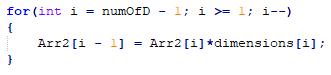
\includegraphics[scale = 1]{code.png}
		\caption{Excerpt code}
		\label {code}
	\end{figure}

	The result of Figure~\ref{code} is then multiplied with the array that contains the indices which describe the coordinates. The result is a one-dimensional equivalent index of the k-dimensional coordinates. This is a variation of row major ordering but follows similar principles. 

\subsection{Procedure 1}
Procedure 1 is titled ‘initZeros’ and is included in initZeros.h header file. The function takes in the one-dimensional representation, the bounds and the number of dimensions as input arguments. The function then calculates the total number of elements in the array by taking the product of the bounds using a helper function called ‘getArraySize’. The array is then initialised to zeros by iterating through all the elements in the one-dimensional array and setting each value to zero.


\subsection{Procedure 2}
Procedure 2 is titled ‘setOnes’ and is included in the setOnes.h header file. It takes a similar approach to ‘initZeros’. The total number of elements is calculated, and 10\% of that number is then taken. The function then sets the first 10\% of the array to one by iterating through till the 10\% index value.

\subsection{Procedure 3}

This procedure is responsible for generating random indexes in the one-dimensional array finding the value at that index printing it and then  printing the equivalent indices of the K-dimensional array that the one-dimensional array represents. 

This is done using the floor function in <math.h>. The indices are calculated in a for loop that runs as many times as there are dimensions in the K-dimensional array by taking the floor of the quotient of the one-dimensional coordinate and the element in the Arr2 array mentioned above that corresponds to the iteration of the loop. The resulting number is multiplied with the corresponding value in the Arr2 array and the product of those two are subtracted from the original 1D coordinate. This process is repeated until all indices are filled and the result of the subtraction is zero.

This is the process of essentially mapping the one-dimensional array’s coordinate back to the coordinate system of the imaginary K-dimensional array.  

\end{document}
